\documentclass[conference]{IEEEtran}

\usepackage{cite}
\usepackage{amsmath}
\usepackage{graphicx}
\usepackage{booktabs}
\usepackage[section]{placeins}
\usepackage{pgfplots}
\usepackage{siunitx}
\usepackage{url}
\usepgfplotslibrary{statistics}
\pgfplotsset{compat=1.18}

\title{Country-Scale Offline Speed-Limit Inference on Smartphones: A Runtime Data Architecture Study}

\author{
\IEEEauthorblockN{Anonymous Authors}
\IEEEauthorblockA{Submission prepared for double-blind review}
}

\begin{document}
\maketitle

\begin{abstract}
This paper evaluates runtime data architectures for low-latency, offline-capable smartphone speed-limit inference using country-scale OpenStreetMap (OSM) data. We identify four data processing scenarios that are compared to find an optimal query and update scenario along three typical query conditions. Hence, we identify the preferred operating point for practical deployment for on-device speed-limit inference as required for Intelligent speed assistance (ISA) applications that are mandatory for new vehicles in the EU since 2022 and open the way for a smartphone and open data based retrofitting approach for vehicles that are already in traffic. Thereby we can strongly support the EU traffic safety vision of reduced crash severity.
\end{abstract}

\begin{IEEEkeywords}
Intelligent transportation systems, intelligent speed assistance, mobile GIS, OpenStreetMap, spatial indexing, offline-first
\end{IEEEkeywords}

\section{Introduction}
Excessive speed remains a major crash-severity factor, and the deployment of Intelligent Speed Assistance (ISA) is now required in new EU vehicle types \cite{eu2019_2144,eu2021_1958,eu_mandatory_safety_2024}. However, the installed vehicle base is substantially larger than annual new registrations, which motivates retrofit-capable software solutions that can run on smartphones with open geospatial data.

Most map-matching research focuses on inference models under sparse/noisy trajectories. In practical mobile deployment, a separate constraint is often dominant: country-scale map data must be queried with low latency under limited memory, storage I/O, and intermittent connectivity. This paper targets that runtime architecture problem.

The practical motivation is scale. EU passenger-car stock remains above 260 million vehicles, whereas annual registrations are only a fraction of that stock \cite{eurostat_passenger_cars_2026,acea_registrations_2024}. In parallel, smartphone internet usage is high in both urban and rural contexts \cite{eurostat_mobile_internet_2024}, making mobile offline-first assistance a feasible deployment channel for legacy vehicles.

The study is positioned for ITS tracks focused on infrastructure technologies and traffic data systems. The contribution is not a new probabilistic matching model; it is a deployment-oriented comparison of runtime data representations and update behavior for speed-limit inference.

\textbf{Contributions:}
\begin{enumerate}
\item A controlled comparison of four country-scale runtime architectures (S1--S4) built from identical source data.
\item Joint latency evaluation for cloud-like host execution and physical smartphone execution across three query modes.
\item A 30-day daily-diff update analysis to compare maintenance effort and update locality.
\item A deployment recommendation balancing query latency and incremental update cost.
\end{enumerate}

\section{Related Work}
Map matching for transport applications has been widely studied, including geometric/topological methods \cite{quddus2007} and probabilistic sequence models such as HMM-based approaches \cite{newson2009,lou2009,goh2012,he2013}. Later work improved robustness for sparse trajectories and route-level inference \cite{rahmani2013,hunter2014,quddus2015,jagadeesh2017,che2018}.

This paper complements that line of work by isolating the systems layer around map data packaging and spatial access. R-tree indexing \cite{guttman1984} is treated as an established mechanism whose deployment characteristics are compared across architecture variants.

Compared with prior ITS map-matching studies, the design focus here is on country-scale runtime packaging and update operability, not only per-query geometric accuracy. This positioning is relevant to production constraints in connected and non-connected operation: an architecture that is fast in a server benchmark may fail under mobile sandbox I/O constraints, while a compact architecture can preserve both latency and maintainability.

\section{Technical Vision}
The technical vision for our research project is an offline-first ISA retrofit platform that can scale from map consumption to crowd-supported map maintenance without requiring user accounts. The initial runtime knowledge base is built from OpenStreetMap and regulatory datasets, then released as immutable artifacts for cloud distribution and smartphone-local execution. On device, location and heading signals are processed by a low-latency inference engine against the local baseline runtime database to produce speed-limit context under intermittent or absent connectivity.

\begin{figure*}[!t]
\centering
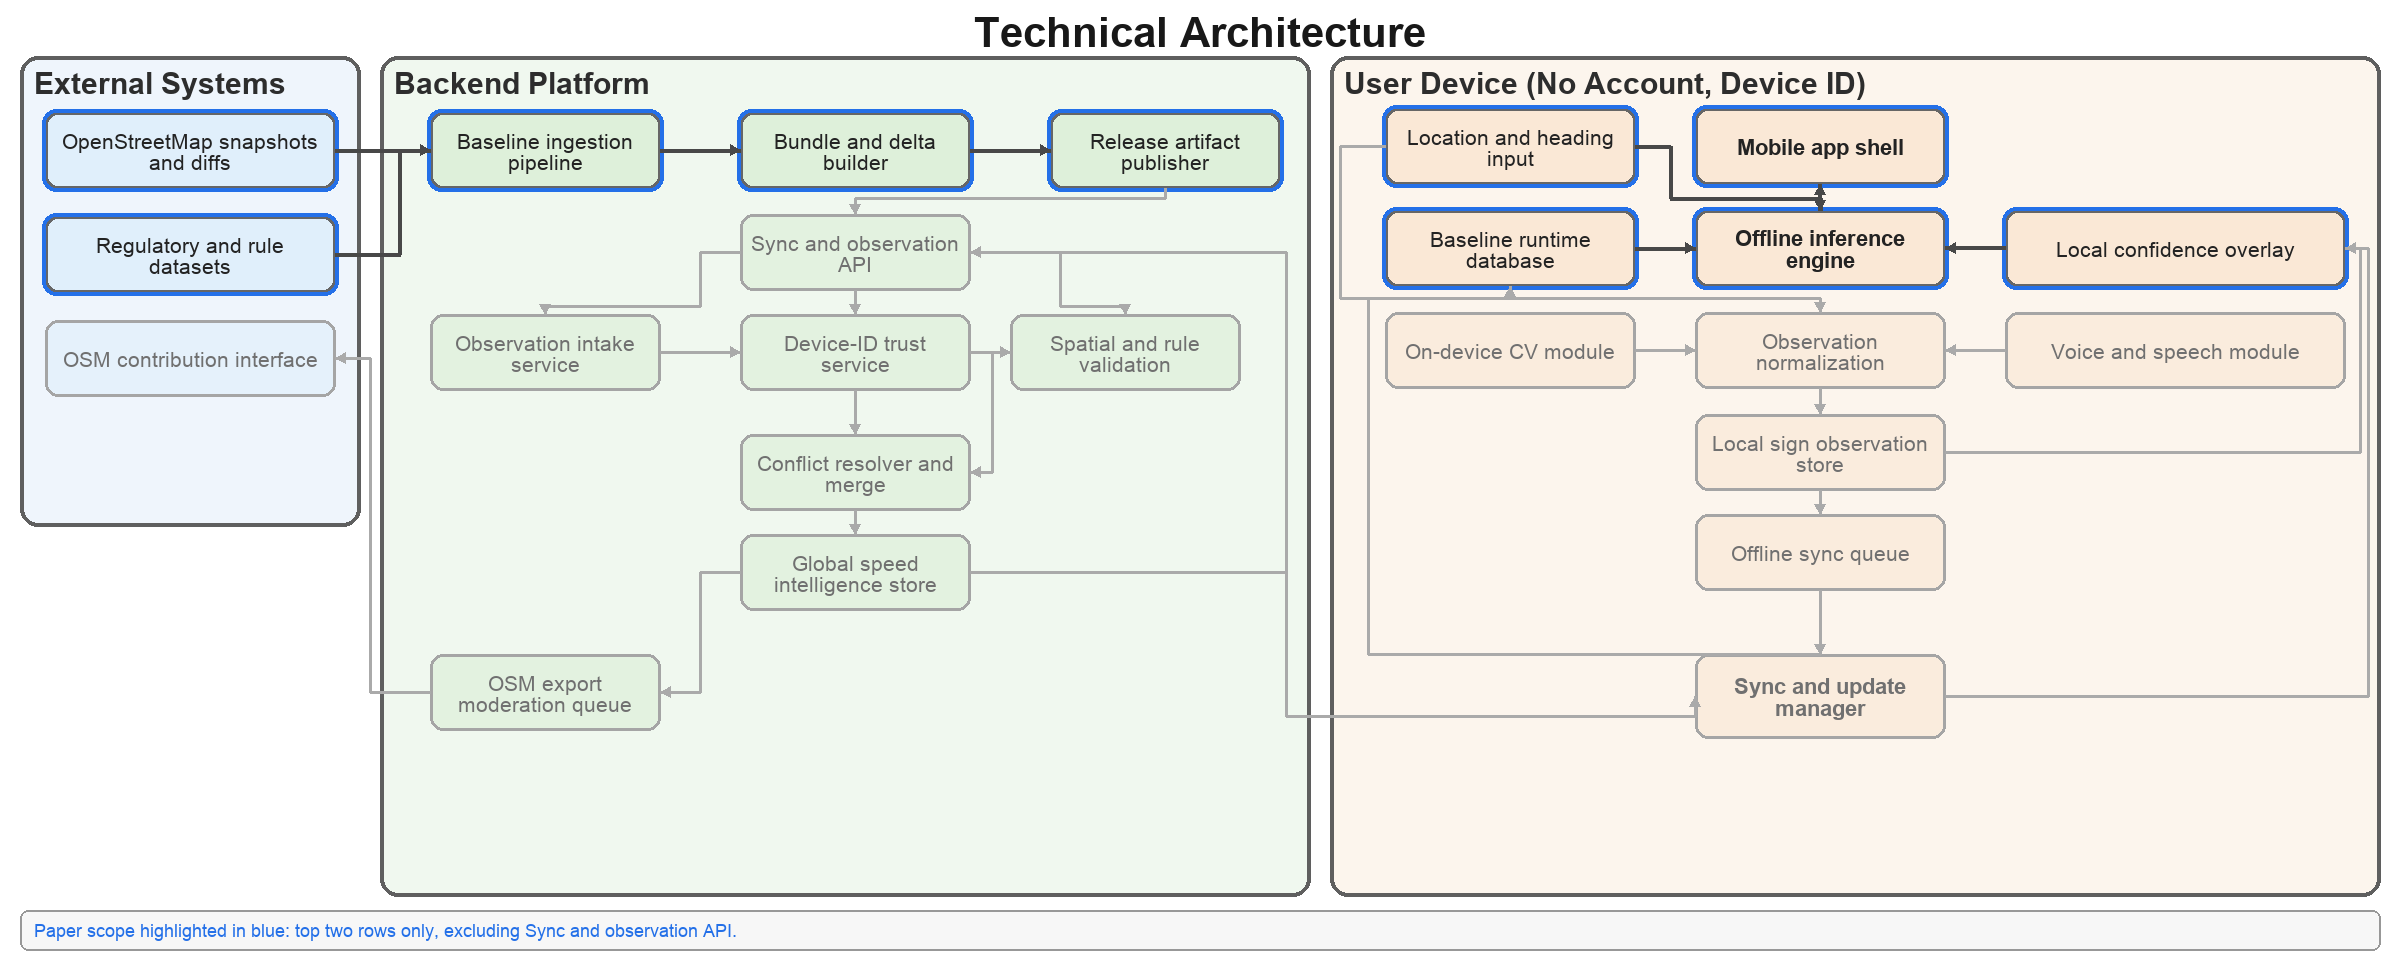
\includegraphics[width=0.98\textwidth,trim=18 470 18 18,clip]{../share/TECHNICAL_ARCHITECTURE_PAPER_SCOPE_BLIND.png}
\caption{Paper-scope technical architecture. Blue highlights indicate the part evaluated in this manuscript (top two rows, excluding the Sync and observation API).}
\label{fig:tech_vision_scope}
\end{figure*}

The long-term extension is a local-first observation loop. Drivers can contribute potential speed-sign updates through voice input and on-device computer-vision capture when road view is available. Observations are normalized locally, stored with pseudonymous device-ID context, and queued for deferred synchronization. The backend then applies spatial and rule validation, resolves conflicts, and merges accepted updates into the global speed intelligence store, with an optional moderated export path to external map ecosystems.

This creates two coordinated loops: a baseline update loop from authoritative sources and an observation loop from user devices. Figure~\ref{fig:tech_vision_scope} highlights the paper scope in blue. The methodology in the next section is intentionally restricted to that scope: country-scale baseline preparation, runtime data packaging scenarios, and on-device inference query behavior. The lower sync-observation stack is architecturally specified but not benchmarked in this manuscript.

\section{Methodology}
\subsection{Data scope and regulatory baseline}
All scenarios use the same OSM Germany snapshot (\texttt{germany-latest.osm.pbf}, \SI{4.70}{GB}) \cite{geofabrik2026}. Preprocessing retains car-drivable \texttt{highway=*} classes and associated speed annotations. Table~\ref{tab:data_profile_provenance} combines dataset profile statistics with speed-limit provenance after rule-aware fusion \cite{osmwiki_highways,osmwiki_maxspeed}.

When explicit speed tags are absent, the legal default baseline for Germany (\SI{50}{km/h} urban, \SI{100}{km/h} rural) is applied \cite{stvo_3}. This rule-aware fallback is necessary because most ways do not carry explicit speed tags.

\begin{table}[!t]
\caption{Combined dataset profile and speed-limit provenance (Germany snapshot).}
\label{tab:data_profile_provenance}
\centering
\begin{tabular}{p{4.8cm}r}
\toprule
Metric & Value \\
\midrule
Input file size & \SI{4.70}{GB} \\
Car-drivable ways & 7{,}963{,}481 \\
\texttt{maxspeed=*} ways & 2{,}637{,}020 \\
\texttt{zone:maxspeed=*} ways & 172{,}116 \\
Explicit speed-limit ways & 2{,}639{,}693 \\
Area-context objects & 129{,}459 \\
\midrule
Explicit tagged limit (share) & 33.15\% \\
Implicit regulatory tag (share) & 0.98\% \\
Default-rule fallback (share) & 65.87\% \\
\bottomrule
\end{tabular}
\end{table}

\subsection{Runtime architecture scenarios}
The four scenarios reflect distinct deployment trade-offs. S1 is a global-index baseline that queries country-scale index files directly. Its implementation is simple, but each lookup can trigger broader scans and higher I/O pressure. S2 introduces explicit spatial partitioning with content-addressed tiles. This localizes reads to relevant map partitions and supports selective tile-level refresh when updates arrive. S3 shifts to a single-file embedded database with spatial indexing; query execution performs direct spatial-window retrieval followed by geometric ranking, reducing candidate fan-out and simplifying deployment to one artifact. S4 adds a tile-membership prefilter before spatial-index intersection, aiming to prune dense urban candidate sets at the cost of an additional filtering stage.

For deployment, S2--S4 use immutable file artifacts per build and are therefore suitable for object-storage distribution, stateless worker replication, and autonomous offline execution on mobile devices.

\subsection{Query modes}
All scenarios share the same ranking score:
\begin{equation}
\text{score} = d + \lambda_h \cdot \Delta \theta + p_u
\label{eq:score}
\end{equation}
where \(d\) is the geometry distance term, \(\Delta \theta\) is bidirectional heading mismatch, \(\lambda_h\) is heading weight, and \(p_u\) is an optional unknown-highway penalty.

The three query scenarios are designed to cover practical operating modes for moving-vehicle inference:
\begin{itemize}
\item \textbf{\texttt{bbox}:} \(d\) is computed from haversine distance to the clamped point on each candidate bounding box. This is the fastest approximation and acts as a coarse candidate filter.
\item \textbf{\texttt{polyline}:} \(d\) is computed as minimum point-to-segment distance over full candidate geometry. This provides the highest geometric fidelity, especially on curved and elongated segments.
\item \textbf{\texttt{hybrid}:} candidates are first ranked by \texttt{bbox}; a limited top-\(N\) subset is then refined using \texttt{polyline}. This aims to preserve near-\texttt{polyline} quality while reducing compute cost.
\end{itemize}

These scenarios capture a practical latency-fidelity spectrum and are evaluated identically for all runtime architectures.

\subsection{Update analysis protocol}
Incremental behavior is evaluated over a 30-day daily-diff window (2026-01-22 to 2026-02-20). The analysis measures changed ways, speed-tag changes, and scenario-specific refresh effort proxies (partition invalidation for S1/S2; simulated patch runtime for S3/S4).

The update protocol uses daily replication deltas to approximate operational maintenance effort between full snapshot checkpoints. This allows comparing granular partition invalidation (S1/S2) with patch-like database updates (S3/S4) under the same observation horizon.

\section{Experimental Setup}
Two deployment contexts are measured:
\begin{itemize}
\item \textbf{Cloud-like host:} MacBook Pro (Apple M4 Max, 48 GB RAM), macOS 15.5.
\item \textbf{Offline device:} physical iPhone 14 Pro (iOS 26.2.1), data stored in mobile sandbox.
\end{itemize}

The benchmark uses a fixed Berlin probe point (\(52.5200,13.4050\)), heading \(90^\circ\), top-\(k=5\), and all three query modes.

Runtime footprint differs substantially by architecture: S1 uses 7 files (\SI{5.09}{GB}), S2 uses 109{,}333 files (\SI{4.61}{GB}), S3 uses 1 file (\SI{2.60}{GB}), and S4 uses 1 file (\SI{3.00}{GB}).

\section{Results}
\subsection{Latency comparison}
Table~\ref{tab:bench_joint} reports mean latencies (ms) across deployment contexts and query modes, while Figure~\ref{fig:bench_boxplot} presents the same matrix in scenario-first view.

\begin{table}[!t]
\caption{Mean latency matrix (\si{\milli\second}) at the benchmark coordinate.}
\label{tab:bench_joint}
\centering
\footnotesize
\setlength{\tabcolsep}{3pt}
\begin{tabular}{lrrrr}
\toprule
Mode & S1 & S2 & S3 & S4 \\
\midrule
\multicolumn{5}{l}{\textbf{Online (cloud-like)}} \\
\texttt{bbox}     & 4815.67 & 187.28 & 84.39 & 63.28 \\
\texttt{hybrid}   & 8306.77 & 179.32 & 27.03 & 67.77 \\
\texttt{polyline} & 8367.55 & 165.19 & 35.99 & 76.33 \\
\midrule
\multicolumn{5}{l}{\textbf{Offline (device)}} \\
\texttt{bbox}     & 3970.84 & 194.49 & 37.12 & 757.01 \\
\texttt{hybrid}   & 2535.44 & 45.76 & 23.39 & 95.96 \\
\texttt{polyline} & 2639.76 & 62.88 & 44.93 & 86.48 \\
\bottomrule
\end{tabular}
\end{table}

S3 is the strongest overall device configuration for decision-relevant query modes (\texttt{hybrid}, \texttt{polyline}). Compared with S1, host-side speedups reach \(307.3\times\) (S3, \texttt{hybrid}). On device, the ordering remains \(S3 < S2 < S4 \ll S1\) for \texttt{hybrid} and \texttt{polyline}.

An important observation is that S4 does not uniformly dominate S3. While S4 applies additional prefiltering intended to reduce dense-area fan-out, the extra stage increases overhead in some device-side conditions, including the \texttt{bbox} mode where S4 regresses strongly versus S3. This indicates that multi-stage filtering needs workload-specific tuning and is not automatically beneficial.

To translate latency into a raw location-update budget, the following relation is used:
\begin{equation}
f_{\text{query}}=\frac{1000}{t_{\text{ms}}}, \qquad
v_{\max}=3.6\cdot f_{\text{query}} \cdot \Delta s
\label{eq:speed}
\end{equation}
where \(t_{\text{ms}}\) is mean latency and \(\Delta s=\SI{10}{m}\) is the inter-fix spacing assumption.

\begin{table}[!t]
\caption{On-device throughput envelope from measured latency.}
\label{tab:device_speed_envelope}
\centering
\begin{tabular}{lrrrr}
\toprule
Scenario & Mean ms & Hz & Best \(v_{\max}\) & Worst \(v_{\max}\) \\
\midrule
S1 & 3048.68 & 0.33 & 14.2 & 9.1 \\
S2 & 101.04 & 9.90 & 786.7 & 185.1 \\
S3 & 35.15 & 28.45 & 1539.1 & 801.2 \\
S4 & 313.15 & 3.19 & 416.3 & 47.6 \\
\bottomrule
\end{tabular}
\end{table}

\subsection{Incremental update workload}
Table~\ref{tab:update_summary} summarizes daily-diff update effort, and Figure~\ref{fig:monthly_updates} shows daily dynamics for additions, removals, and speed-tag changes.

\begin{table}[!t]
\caption{30-day daily-diff update summary (2026-01-22 to 2026-02-20).}
\label{tab:update_summary}
\centering
\begin{tabular}{p{4.8cm}rr}
\toprule
Metric & Total & Mean/day \\
\midrule
Changed ways (\(+\), \(-\), modified) & 1{,}829{,}171 & 60{,}972 \\
\texttt{maxspeed}-related tag changes & 139{,}999 & 4{,}667 \\
Invalidated S1 grid cells & 201{,}355 & 6{,}712 \\
Invalidated S2 tiles & 80{,}536 & 2{,}685 \\
S3 simulated patch runtime & \SI{30719.38}{ms} & \SI{1023.98}{ms} \\
S4 simulated patch runtime & \SI{40710.02}{ms} & \SI{1357.00}{ms} \\
\bottomrule
\end{tabular}
\end{table}

S2 improves refresh locality versus S1 (fewer invalidated partitions), while S3 is more efficient than S4 among database-centered variants (\(1.33\times\) lower mean patch runtime).

To estimate practical mobile transfer costs, payload transmission time is modeled as:
\begin{equation}
T=\frac{B_{\text{payload}}+B_{\text{overhead}}}{R}
\end{equation}
with \(B_{\text{overhead}}=0.1 \cdot B_{\text{payload}}\). For European 5G conditions, \(R\) is bounded by reported ranges in recent network measurements \cite{opensignal_europe_5g_2024,eu_connectivity_impact_2026}. Under this model, compact SQL patch transfer for S3 remains faster than broad tile-bundle refresh for S2 at equivalent daily coverage.

\begin{table}[!t]
\caption{Indicative update transfer times under measured daily volumes.}
\label{tab:transfer}
\centering
\begin{tabular}{p{3.5cm}r}
\toprule
Case & Transfer time (s) \\
\midrule
S2: 100 median tiles (\SI{4.72}{MB}) & 0.19--0.40 \\
S2: 1000 median tiles (\SI{47.2}{MB}) & 1.91--3.98 \\
S2: mean daily invalidation (\SI{126.73}{MB}) & 5.13--10.69 \\
S3: daily SQL patch (\SI{5.07}{MB}) & 0.21--0.43 \\
\bottomrule
\end{tabular}
\end{table}

\subsection{Deployment choice and track relevance}
Under equal weighting of query latency and update effort, S3 is the preferred operating point. The architecture provides low-latency on-device lookup, compact single-file deployment, and lower incremental update overhead than S4.

For ITSC positioning, this evidence primarily supports tracks in \emph{Infrastructure and ITS Technologies} and \emph{Traffic Data Analytics and Machine Learning}, with secondary relevance for \emph{ITS Validation and Verification}.

\section{Threats to Validity}
The benchmark uses one fixed probe location and heading, and therefore does not represent all geometric or traffic contexts. The update analysis uses one 30-day window and should be extended with longer seasonal coverage. Finally, the current evaluation reports latency and update effort but does not yet include end-to-end driving-assistance effectiveness metrics in fleet-scale trials.

\section{Conclusion}
This paper evaluated four runtime data architectures for country-scale, offline-capable speed-limit inference on smartphones. Keeping source data and query logic constant isolates architecture effects: global indexes (S1) are not viable for low-latency mobile deployment, tiled packs (S2) improve locality, and embedded spatial databases dominate latency. Among embedded variants, S3 provides the best latency-update tradeoff and is selected as the default architecture for practical deployment.

Future work will extend the benchmark to route-level workloads, multi-country datasets, and longitudinal weekly checkpoints with intervening daily diffs.

\section{Reproducability}
All preprocessing, scenario construction, and benchmark steps are parameterized and versioned in the accompanying research codebase available at \url{https://github.com/}. The evaluation reported here is tied to the Germany snapshot dated 2026-02-23, with fixed probe location, heading, query modes, and scenario definitions stated in the methodology and evaluation sections. 

\bibliographystyle{IEEEtran}
\bibliography{../share/IEEEabrv,../share/references}
\appendices
\section{Evaluation Figures}

\begin{figure*}[!t]
\centering
\begin{tikzpicture}
\begin{axis}[
  ybar,
  width=0.95\textwidth,
  height=0.24\textheight,
  bar width=4pt,
  ylabel={Latency (ms, log scale)},
  ymode=log,
  ymin=10,
  ymax=10000,
  xmin=0.5,
  xmax=8.5,
  xtick={1,2,3,4,5,6,7,8},
  xticklabels={S1 online,S1 offline,S2 online,S2 offline,S3 online,S3 offline,S4 online,S4 offline},
  xticklabel style={rotate=30,anchor=east,font=\scriptsize},
  legend style={at={(0.5,1.04)},anchor=south,legend columns=3,font=\small},
  ylabel near ticks,
  grid=major
]
\addplot coordinates {
  (1,4815.67) (2,3970.84) (3,187.28) (4,194.49)
  (5,84.39) (6,37.12) (7,63.28) (8,757.01)
};
\addplot coordinates {
  (1,8306.77) (2,2535.44) (3,179.32) (4,45.76)
  (5,27.03) (6,23.39) (7,67.77) (8,95.96)
};
\addplot coordinates {
  (1,8367.55) (2,2639.76) (3,165.19) (4,62.88)
  (5,35.99) (6,44.93) (7,76.33) (8,86.48)
};
\draw[gray,densely dashed,thick] (axis cs:2.5,10) -- (axis cs:2.5,10000);
\draw[gray,densely dashed,thick] (axis cs:4.5,10) -- (axis cs:4.5,10000);
\draw[gray,densely dashed,thick] (axis cs:6.5,10) -- (axis cs:6.5,10000);
\legend{bbox,hybrid,polyline}
\end{axis}
\end{tikzpicture}
\caption{Scenario-first latency view. For each scenario (S1--S4), online and offline columns are adjacent; dashed lines delimit scenario groups.}
\label{fig:bench_boxplot}
\end{figure*}

\begin{figure*}[!t]
\centering
\begin{tikzpicture}
\begin{axis}[
  width=0.95\textwidth,
  height=0.24\textheight,
  xlabel={Date (UTC)},
  ylabel={Count/day},
  xmin=1,
  xmax=30,
  ymin=0,
  ymax=27000,
  xtick={1,4,7,10,13,16,19,22,25,28},
  xticklabels={01-22,01-25,01-28,01-31,02-03,02-06,02-09,02-12,02-15,02-18},
  xticklabel style={rotate=30,anchor=east,font=\scriptsize},
  ymajorgrids=true,
  grid style={gray!25},
  legend style={at={(0.02,0.98)},anchor=north west,font=\scriptsize,fill=none,draw=none},
  ylabel near ticks
]
\addplot[thick,color={rgb,255:red,27;green,158;blue,119}] coordinates {(1,18013) (2,19254) (3,18260) (4,17438) (5,21334) (6,24457) (7,23643) (8,22933) (9,21015) (10,16429) (11,14368) (12,16727) (13,19650) (14,19698) (15,16405) (16,17607) (17,16965) (18,15923) (19,19745) (20,23371) (21,21608) (22,19435) (23,19166) (24,18455) (25,18826) (26,19617) (27,17806) (28,16920) (29,17859) (30,17969)};
\addplot[thick,color={rgb,255:red,217;green,95;blue,2}] coordinates {(1,1900) (2,1937) (3,1782) (4,1747) (5,1853) (6,2117) (7,2201) (8,1885) (9,1702) (10,1541) (11,1413) (12,1756) (13,2702) (14,2526) (15,4186) (16,4405) (17,1693) (18,1323) (19,1475) (20,1969) (21,2012) (22,1936) (23,1872) (24,1795) (25,1786) (26,1936) (27,3133) (28,2973) (29,1735) (30,2180)};
\addplot[thick,color={rgb,255:red,117;green,112;blue,179}] coordinates {(1,4212) (2,4148) (3,4556) (4,5214) (5,5037) (6,4353) (7,4596) (8,4683) (9,4603) (10,4868) (11,5615) (12,5668) (13,4810) (14,5071) (15,4701) (16,4029) (17,4915) (18,5310) (19,4822) (20,4997) (21,4906) (22,4330) (23,4009) (24,4185) (25,4223) (26,4496) (27,4237) (28,3894) (29,4465) (30,5046)};
\legend{ways added,ways removed,maxspeed changes}
\end{axis}
\end{tikzpicture}
\caption{Daily update dynamics over the 30-day analysis window.}
\label{fig:monthly_updates}
\end{figure*}

\end{document}
